\frnote{ret}
The people that uses a system can be represent by personas. This is done in order to ensure the PACT elements are in center in the design process. Personas are profiles of different types of users that will use the system. A persona is a concrete representations of a fictitious person. Personas helps the designer design for a person in there mind and prevent that the the system is designed for themselves. Personas are developed through the understanding process and through undertaking a PACT analysis. A part of the persona is a short story of the person trying to achieve a goal using the system in a context \cite{benyon2013designing}.

As part of the project one persona was made, based on %\cref{interviewbruger}.
This is camilla an average user of the system.

\subsubsection{Camilla}
\begin{figure} [h]
  \centering
  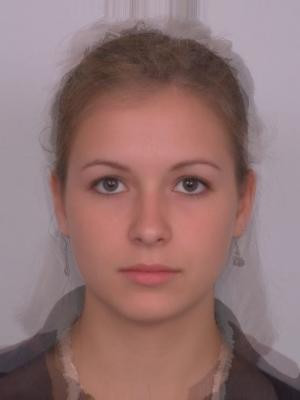
\includegraphics[]{Images/average.jpg}
  \caption{Picture associated with the persona Camilla. Copyright the Face Research Lab. Used with permission.}
  \label{fig:camilla}
\end{figure}
\begin{itemize}
\item 25 years old
\item Medical student
\item Employed in an elderly care center
\item In a relationship with Keith
\item She loves meeting new people
\item When going out she likes to visit small places that allow socialisation
\item Volunteered in Red Cross Uganda
\end{itemize}

It is friday afternoon and Camilla is planning to meet some of her fellow students at a bar. Camilla and her friends get together after they are finished at school and go to a café to grab a sandwich. After dinner, Camilla takes out her smartphone and checks openPlaylist. Camilla can see that some of her favorite songs are being played at White Hart, and they agree to go there. Upon arriving Camilla checks in via the app. She immediately notices on the screen behind the bar that the queue is filled with songs she dislikes. She now uses the app to request and upvote other songs that she would like to be played. Some other people at White Hart agree on Camilla's choices and they too upvote these songs. On the screen in the bar Camilla can see some of the other people that upvotes her songs and later in the evening she meets them and they talk about all the nice music they have in common. Camilla and her new and old friends party all night long and drink a lot of beer.